%----------------------------------------------------------------------------------------
%	PACKAGES AND OTHER DOCUMENT CONFIGURATIONS
%----------------------------------------------------------------------------------------
\PassOptionsToPackage{unicode=true}{hyperref} % options for packages loaded elsewhere
\PassOptionsToPackage{hyphens}{url}
%
\documentclass[11pt]{article}
\usepackage{appendix}
\usepackage{lmodern}
\usepackage{amssymb,amsmath}
\usepackage{ifxetex,ifluatex}
%-------%
% Journal submission specifications - ASA format
%\usepackage{mathptmx}
%\usepackage[,bottom=1in,top=1in,left=1in,right=1in]{geometry}
\usepackage{geometry}
%\usepackage[doublespacing]{setspace} % alternate way to add double space
%\usepackage[document]{ragged2e} % do not right-justify text
%\usepackage{enotez}
%  \let\footnote=\endnote

%Running header
\usepackage{fancyhdr}
\pagestyle{fancy}
\fancyhf{}% Clear header/footer
\fancyhead[L]{Paying Attention to the Pandemic}
%\cfoot{\thepage} %page numbers bottom center
\rhead{\thepage} %page number right side header
\cfoot{}

% where figures/tables in document
%\usepackage[nolists,tablesfirst]{endfloat} % forces all floats to appear at end of document
\usepackage[section]{placeins} %keeps floats in place, using command \FloatBarrier
%\usepackage[nolists, tabhead, fighead]{endfloat}
%\usepackage{flafter} %force floats to appear after they are defined
%-------%

 % packages for figures
\usepackage{array}  % tables
\usepackage{wrapfig}  % wrap text around narrow tables or figures
\usepackage{graphicx}  % for inserting graphics from file
\usepackage{blindtext}
\usepackage{asymptote}
\usepackage{subcaption}
\usepackage{rotating} %landscape tables
\usepackage{geometry}
\usepackage{pdflscape}

%--------
% For Tables created by estout
\newcommand{\sym}[1]{\rlap{$#1$}} % for symbols in Table
\usepackage{siunitx}
\sisetup{ detect-mode,
          group-digits            = false ,
          input-signs             = ,
          input-symbols           = ()[]-+* , % specifying \sym here does not work
          input-open-uncertainty  = ,
          input-close-uncertainty = ,
          table-align-text-post   = false
        }

\def\xxx#1{%
  \bgroup\uccode`\~\expandafter`\string#1%
  \uppercase{\egroup\edef~{\noexpand\text\string#1}}%
  \mathcode\expandafter`\string#1"8000 }
\def\textsymbols{\xxx[\xxx]\xxx(\xxx)\xxx*}

\makeatletter
\edef\originalbmathcode{%
    \noexpand\mathchardef\noexpand\@tempa\the\mathcode`\(\relax}
\def\resetMathstrut@{%
  \setbox\z@\hbox{%
    \originalbmathcode
    \def\@tempb##1"##2##3{\the\textfont"##3\char"}%
    \expandafter\@tempb\meaning\@tempa \relax
  }%
  \ht\Mathstrutbox@\ht\z@ \dp\Mathstrutbox@\dp\z@
}
\makeatother

\usepackage{changepage} % allows to use \begin{adjustwidth} to shift margins for table
%--------

% for figures in multiple parts
\usepackage{caption}
%\DeclareCaptionLabelFormat{cont}{#1~#2\alph{ContinuedFloat}}
%\captionsetup[ContinuedFloat]{labelformat=cont}

%Bibliography
\usepackage{natbib}
\setcitestyle{round,aysep={},yysep={,},notesep={:}}


\ifnum 0\ifxetex 1\fi\ifluatex 1\fi=0 % if pdftex
  \usepackage[T1]{fontenc}
  \usepackage[utf8]{inputenc}
  \usepackage{textcomp} % provides euro and other symbols
\else % if luatex or xelatex
  \usepackage{unicode-math}
  \defaultfontfeatures{Ligatures=TeX,Scale=MatchLowercase}
\fi
% use upquote if available, for straight quotes in verbatim environments
\IfFileExists{upquote.sty}{\usepackage{upquote}}{}
% use microtype if available
\IfFileExists{microtype.sty}{%
\usepackage[]{microtype}
\UseMicrotypeSet[protrusion]{basicmath} % disable protrusion for tt fonts
}{}
\IfFileExists{parskip.sty}{%
\usepackage{parskip}
}{% else
\setlength{\parindent}{0pt}
\setlength{\parskip}{6pt plus 2pt minus 1pt}
}
\usepackage{hyperref}
\hypersetup{
            pdftitle={Knowledge of COVID-19 and News Sources},
            pdfborder={0 0 0},
            breaklinks=true}
\urlstyle{same}  % don't use monospace font for urls
\usepackage{graphicx,grffile}
\makeatletter
\def\maxwidth{\ifdim\Gin@nat@width>\linewidth\linewidth\else\Gin@nat@width\fi}
\def\maxheight{\ifdim\Gin@nat@height>\textheight\textheight\else\Gin@nat@height\fi}
\makeatother
% Scale images if necessary, so that they will not overflow the page
% margins by default, and it is still possible to overwrite the defaults
% using explicit options in \includegraphics[width, height, ...]{}
\setkeys{Gin}{width=\maxwidth,height=\maxheight,keepaspectratio}
\setlength{\emergencystretch}{3em}  % prevent overfull lines
\providecommand{\tightlist}{%
  \setlength{\itemsep}{0pt}\setlength{\parskip}{0pt}}
\setcounter{secnumdepth}{0}
% Redefines (sub)paragraphs to behave more like sections
\ifx\paragraph\undefined\else
\let\oldparagraph\paragraph
\renewcommand{\paragraph}[1]{\oldparagraph{#1}\mbox{}}
\fi
\ifx\subparagraph\undefined\else
\let\oldsubparagraph\subparagraph
\renewcommand{\subparagraph}[1]{\oldsubparagraph{#1}\mbox{}}
\fi

% set default figure placement to htbp
\makeatletter
\def\fps@figure{htbp}
\makeatother

%----------------------------------------------------------------------------------------
%	DOCUMENT CONTENT
%----------------------------------------------------------------------------------------

\begin{document}

\title{Paying Attention to the Pandemic: \\ Knowledge of COVID-19 by News Sources and Demographics}

\author{} 
\date{}

\clearpage\maketitle

%----------------------------------------------------------------------------------------
\section{Abstract}\label{sec:abstract}
%----------------------------------------------------------------------------------------
\pagestyle{fancy} %Running header
\setcounter{page}{1} %resets page number to 1

Previous research has looked at the role of social media and other news sources on shaping the U.S. population?s understanding of the COVID-19 pandemic. However, what has not been studied is how this knowledge acquisition is structured by the demographic characteristics of gender, race and ethnicity, income, and education. This study reveals how the use of different news sources differentially shapes access to accurate information about COVID-19 and related topics for different demographics. I answer these questions by analyzing recent Pew Research survey data asking respondents about their news media consumption and their knowledge of COVID-19 science and related current events information. I determine the effect of demographic group memberships in shaping knowledge about COVID-19 received through news sources.
 
\section{Keywords}

knowledge, inequality, media, COVID-19

\newpage

%----------------------------------------------------------------------------------------
\section{Introduction}\label{sec:introduction}
%----------------------------------------------------------------------------------------

Given the rapidly developing landscape of knowledge about COVID-19, as well as the importance of the disease in people's lives, nine in ten Americans say they are following news about the outbreak very or fairly closely.\footnote
    {See Appendix Table~\ref{table:followClosely}.} 
Having up-to-date, accurate knowledge of science and public health policy has consequences not only for one's own health, but also for the well-being of one's family and community. Yet the challenges in sorting through this information are perhaps greater than ever \citep{Metaxa-Kakavouli2017}. This paper investigates how demographic categories and news source influence accurate understanding of the facts about COVID-19. This research has implications for sociology, media, and information studies. 


%-------------------------
\subsection{Information Inequalities}

Many prior studies have evaluated information seeking behaviors and needs \citep{Case2016}. Broadly speaking, there are two reasons why we might be concerned about differential access to correct facts:

\begin{enumerate}
\def\labelenumi{(\arabic{enumi})}
\item
  Differences in the amount of information people have are influenced by unequal social positions in our society; and
\item
  Accurate information is a potential source of later inequality in outcomes.
\end{enumerate}

Researchers have sought to understand which factors contribute to gaps in information and the resulting states of advantage and disadvantage. For a person to be informationally advantaged, they need not only the economic capital for information access, but also the intellectual resources for information gathering, processing, and assessment \citep{Sweetland1993}. In this way, information filtering skills are key. Information overload, in certain contexts, can thus create information poverty rather than making people information rich \citep{Yu2006}. Skill spillovers from knowledge work to personal life may give some groups more abilities than others. Those who use information sorting skills in their occupations may be more able to use these abilities to benefit their private lives, as well \citep{Edwards2000,Xanthopoulou2012}. This may be particularly true in sorting through misinformation in rapidly developing news environments, such as that with the current coronavirus pandemic. 

The information divide results from inequalities in ``the possession and usage of information and communication sources in a particular society'' \citep[231]{Yu2006}. Information inequalities are the product of the unequal distributions of information resources. Information poverty results from this state of deprivation for those in less advantaged positions, based on an interrelated set of knowledge, information, and information infrastructures \citep{Britz2004}. Where might systematic variations in the distribution of information by demographic characteristics come from? Understanding the causes at the root of knowledge differences can point to systemic inequities in the consumption of information, such as those that result from the media.


%-------------------------
\subsection{Inequalities \& Information Consumption}

Understanding the influence of demographic status characteristics and the media on factual information inequality helps us understand the state of knowledge in the U.S.; it also lays the groundwork for the study of potential causes. Here I briefly review relevant research on information acquisition through news aggregators and search engines, social networks and social media, and more traditional TV, print, and radio news. I also discuss briefly what we know about different groups' information seeking patterns through these media during the pandemic. 

Mobile news aggregators like Google News and Apple News are increasingly important forces in the media landscape; about 17\% of people get their news from Google News \citep{Reuters2020}. The distribution of attention on the internet concentrates attention on fewer sites each year, creating an effective size of fewer than 20,000 websites and increasing the Gini coefficient \citep{McCurley2007}. Furthermore, research on algorithmic bias reveals widespread implicit and explicit discrimination \citep{Sweeney2013,ONeil2016,Eubanks2018,Noble2018}. At the same time, while Google does alter its search and news results based on location \citep{KlimanSilver2015,Fischer2020}, it does not appear to do so on ideological grounds \citep{Haim2018}. Email is also an increasingly important format, with one in five Americans accessing an newsletter update direct from a news publisher each week, and half of these reporting it was their primary way of accessing news \citep{Reuters2020}. 

Information also spreads through social networks online. Contrary to widespread opinion, however, engagement with news on Facebook is more limited by user preferences for ideologically homogenous content than by the platform's algorithms \citep{Bakshy2015}. People ``are probabilistically influenced to adopt the opinions of their neighbors, and can promote their own opinions by being reluctant to change them. In this way, an intransigent minority can convert the entire group over to their minority opinion'' \citep{West2011}. Strongly opinionated minority group members can have a strong influence in the information ecosystem of the World Wide Web. In short, psychological and cognitive biases \citep{DiMaggio1997} are colliding with the technological realities of our time to create novel knowledge inequities \citep{Mohammed2012}. Nearly one in two Americans seeks out news on social media websites \citep{Reuters2020}. Many people consume news from Facebook-affiliated social companies, including 35\% from Facebook, 9\% from Facebook Messenger, and 4\% from WhatsApp \citep[87]{Reuters2020}. About one in five people in the U.S. turn primarily to social media for their political news, and these tend to be the least engaged and knowledgeable about coronavirus news \citep{Mitchell2020a}. An increasing proportion of Americans (24\%) also get their news from YouTube \cite{Shearer2017,Reuters2020}.

Among TV, radio and print consumers, 28\% of Americans reported getting their news from local TV news, and only 18\% from a local or regional newspaper, on a weekly basis \citep{Reuters2020}. Only 14\% reported weekly use of a local television news website and 9\% of a regional or local newspaper website \citep{Reuters2020}. This may be partly due to difficulties discovering local news online because Google's search returns favor a small number of large news outlets over local news \citep{Diakopoulos2019,Fischer2020}.

We do know that different demographics are more likely to consume different types of news. For example, older adults follow more local news and more highly educated adults are more likely to follow international news \citep{Mitchell2018}. Local news is viewed as more trustworthy than national news, particularly among Democrats \citep{KnightGallup2019,Reuters2020}. This is confounded by thoroughly documented digital inequalities \citep{Robinson2020a}, which influences what type of news people consume. Those who get their news primarily through local TV and social media are more likely to have lower incomes and less education than those who turn primarily to news websites or apps, cable or network TV, or radio or print news \citep{Mitchell2020a}. This also has implications for who consumes the most misinformation; we do not know how this distribution may differentially affect the information different demographic groups receive about different COVID-19 news topics. 

For example, people who use social media as their most common method of consuming political and election news were the most likely to have heard `a lot' (26\%) about the (false) conspiracy theory that the pandemic was intentionally planned, followed by those who got their news through local TV (20\%) \citep{Mitchell2020a}. Prior to the presidential election, 67\% of U.S. adults reported concern "about what is real and what is fake on the internet" related to news \citep[18]{Reuters2020}. The largest proportion (35\%) reported that they were most concerned about distinguishing misinformation on the Facebook platform \citep[19]{Reuters2020}.


%-political sociology of local news:
%--from fake local news conglomerates
%--decentralized versus centralized new sources
%--what is meaning of friends and family? not getting any news at all?


%-------------------------
\subsection{COVID-19 Knowledge \& Health Outcomes}

Gaps in information produce inequalities in later outcomes. Aside from their role in producing status differences \citep{Ridgeway2014}, differences in knowledge also result in concrete differences in health outcomes. Accurate health knowledge is necessary (though not sufficient) to affect health behavior change \citep{hints11}. For example, in the domain of health, 25\% of Hispanics inaccurately believe that there is nothing people can do to reduce their chances of getting cancer, while only 14\% of non-Hispanic Whites believe this \citep{hints11}. Correct knowledge is a required foundation that is both influenced by and built upon by structural inequalities.

Researchers have looked at the implications of this differential access to accurate information on consequences for health during the COVID-19 pandemic. Those with accurate knowledge about COVID-19 are more likely to have positive health outcomes during the pandemic \citep{Fridman2020}. Early in the pandemic, trust in social media and private news sources was negatively associated with both knowledge about COVID-19 and the practice of social distancing behavior, compared to trust in government information sources \citep{Fridman2020}. On average, U.S. adults indicated they prefer that scientists and government public health leadership manage the response to the COVID-19 pandemic \citep{McFadden2020}. Generally, U.S. adults trust scientists' knowledge about COVID-19; however, this trust varies widely based on demographic characteristics \citep{Evans2020}. It follows that different demographic groups would follow different news sources for emerging information about COVID-19 and the pandemic response.

Demographic characteristics also heavily influence health outcomes from the COVID-19 pandemic. Many would find this normatively problematic if these types of information which historically marginalized groups have the least access to or trust in correspond to the types of information which tend to ensure positive health outcomes. Prior work suggest this is the case, as non-White populations express greater trust in non-government information sources \citep{Fridman2020}.
Because of systemic racism, Black Americans are at greater risk of contracting and dying from COVID-19 \citep{Adegunsoye2020,Kim2020,Millett2020,PriceHaywood2020}.
Older adults are also at much greater risk of infection and mortality from COVID-19 \citep{Ho2020,LeCouteur2020}.
Furthermore, since health management has moved online more than ever during the pandemic \citep{Khilnani2020}, and access to certain digital resources can act as substitutes for in-person interactions \citep{Robinson2020b}, digital inequality is widening existing health and age disparities.
Because of these greater risks, one might expect these demographic groups to more closely follow news about the COVID-19 pandemic; this is the case among Black Americans. 
At least early in the pandemic in spring 2020, Black Americans were more likely to closely follow news about the outbreak and more likely to discuss it with others \citep{Mitchell2020b}. 

%-------------------------
Yet, to my knowledge, no one has yet investigated the consequences of demographic group membership on the joint relationship between differential information acquisition behaviors and knowledge during the COVID-19 pandemic. Therefore, this study investigates how knowledge of the COVID-19 pandemic is structured by the demographic characteristics of gender, race, income, and education. Furthermore, I investigate whether use of different news sources differentially shapes knowledge of current COVID-19 topics based on demographics.


%----------------------------------------------------------------------------------------
\section{Methods}\label{sec:methods}
%----------------------------------------------------------------------------------------

\subsection{Data}\label{sec:data}

In this analysis, I investigate factual knowledge of the pandemic using the Pew Pathways June 2020 American Trends Panel Wave 68 Survey \citep{PewJune2020}. The survey features three questions of particular interest, which ask about factual knowledge about the COVID-19 pandemic:

\begin{enumerate}
\def\labelenumi{(\arabic{enumi})}
  \item ``As far as you know, are antibody tests for the coronavirus (also known as serology tests) intended to detect?'' (Correct answer is ``A previous infection'')
  \item ``Do you happen to know who Anthony Fauci is?'' (Correct answer is ``An infectious disease expert and government health adviser.)'
  \item ``As far as you know, how did states in the U.S. respond during the coronavirus outbreak?''" (Correct answer is ``Some states in the U.S. have not had a statewide stay-at-home order.'')
%  \item ``Is the national unemployment rate as reported by the government currently?'' (Correct answer is 15\%)
\end{enumerate}

My analysis also includes basic demographic variables for respondents, including gender, age, family income, educational attainment, and race. I discuss these in the order they appear in the models. So that readers can see all analysis decisions for themselves, annotated code is available at the Open Science Framework project page: [redacted for blind review].



%-------%
\subsubsection{Gender}\label{sec:gender-vars}

Gender and sex are not binary designations, but rather lie along a flexible
spectrum or at least exist in multiple categories \citep{Connell2002b,
Fausto-Sterling1993, Fausto-Sterling2000, West1987, Maglioizzi2016}.
However, the available data have only categories of `woman' or
`man.' Therefore, I code gender as a binary variable.

%-------%
\subsubsection{Age}\label{sec:age-vars}

Pew provides only categorical age, in predefined groups: 18-29; 30-49; 50-64; and 65 and over. There are, of course, different kinds of things people are expected to know at different life stages. However, there is no reason to expect that the rate of accumulation of knowledge should vary based on any of my other covariates, especially regarding rapidly developing news about the COVID-19 pandemic. Therefore, I include age group as a predictor in my models, but I do not include any squared terms or interaction variables with age.

% Since Pew provides only categorical age, I also use the REDI method
% \citep{KingREDI} to convert age to a continuous variable. I calculate the number % of respondents in each age category, and pull at random an equivalent number of observations within that age range from the CPS ASEC. I take the exact age value  of that observation from the CPS ASEC and assign the age value as if it were the % original respondent's exact age. Again, this preserves variance in the age
% distribution.



%-------%
\subsubsection{Family Income}\label{sec:class-income}

Social class both creates and is produced by differences in knowledge. I use family income and education as measures of social class.\footnote
    {Family income and education are imperfect measures of class, to be sure. Others (such as parental occupation data) would be preferable for both their causal separability\,---\,given the temporal antecedence of parental occupation,\--\,and their empirical validity \citep{Weeden2005a, Weeden2012}. However, parental occupation is not available for these data.}
I choose family income rather than individual (personal) income because it more accurately reflects the total resources available to the individual, and therefore are a better reflection of socioeconomic status.\footnote
  {The reliability of self-reported income typically ranges from 71\% to 98\%, with a mean of 86\% \citep{Marquis1986}. In other words, if the same individuals are asked about their income at two different points in the survey using two slightly different measures to get at the same question, the results will agree, on average, within about 0.86. Compared to tax or Social Security Administration records, self-reported measures of income tend to be about 70  to 78\% of official amounts \citep{Coder1996, Reardon2011a}.}
  
I transform categorical income into continuous income in order to make regression coefficients more interpretable. A continuous measure of income is more intuitive to interpret than categorical income bins. Therefore, I use the Random Empirical Distribution Imputation (REDI) method to convert the Pew categorical family income data into continuous income estimations \citep{KingREDI}. For each category of family income, I randomly draw the same number of observations from within those same bounds in the Current Population Survey March Annual Social and Economic (CPS ASEC) supplement \citep{ASEC2018}. I then apply these exact family income values from the CPS ASEC to the corresponding set of categorical values within the original Pew survey. Thus, I get a distribution of numerical values in the original Pew survey that corresponds to their probability of occurrence in the CPS ASEC. Repeating this for all income categories provides continuous cold-deck imputed income values for every respondent. I used this method rather than assigning the midpoint value to preserve variance and keep information from the extreme income categories. For more details on the conversion of categorical to continuous family incomes, see \citet{KingREDI}.

%https://stats.stackexchange.com/questions/143110/when-to-use-log-in-regression
To aid interpretation, I then take the natural log of this continuous value of family income. Thus, the variable may be interpreted as the impact of a one percent increase in family income on the log odds (or odds) of knowing the correct answer to the question.


%-------%
\subsubsection{Race and Ethnicity}\label{sec:race-and-ethnicity}

Measurement of race is another area in which best practice\footnote
  {Beginning in 2000, the U.S. Census moved from allowing people to choose only one racial category identity to allowing people to choose as many racial categories as they identified with \citep{OfficeofManagementandBudget1997,OfficeofManagementandBudget2000}.}
is often limited by available data. I code the racial categories of non-Hispanic White, non-Hispanic Black/African-American, non-Hispanic Asian, the ethnic category of Hispanics who do not identify with any of the other racial categories, and the category of `other.' This race `pentagon' classification has been found most useful in explaining variation in education and income (compared to either a seven or eight category, tri-racial, or skin tone classification system) \citep{Howell2017}.

In order to simplify the application and interpretation of interaction effects, I also coded a single BIPOC (Black, Indigenous and people of color) variable. This variable includes all respondents that do not identify as non-Hispanic White: Hispanic, Black/African-American, Asian, and other.


%-------%
\subsubsection{Education}\label{sec:education-vars}

Education categories are defined by five categories: less than high school, completed high school, some college, bachelor's degree, and graduate or professional degree. Though education and family income are collinear, education would be expected to have an independent effect on the ability to consume and interpret the news. Therefore, both family income and educational attainment are included in all but the basic models.

%-------%
\subsubsection{News}

The survey asked respondents ``which of these sources do you \emph{rely on most} for news about the coronavirus outbreak?'' \citep{PewJune2020,Shearer2020}. There were ten choices available to respondents:

\begin{enumerate}
\def\labelenumi{(\arabic{enumi})}
    \item International news outlets;
    \item National news outlets;
    \item Local news outlets;
    \item Trump and his coronavirus task force;
    \item Joe Biden and his campaign;
    \item State and local elected officials and their offices;
    \item Public health organizations and officials;
    \item Friends, family and neighbors;
    \item Community or neighborhood newsletters or listserv; and
    \item Online forums or discussion groups.
\end{enumerate}

After initially analyzing the models with all news source categories separate, I grouped news sources together based on their structurally similar roles to facilitate the application of interaction terms and interpretation of results. The sources were combined in the following way: international and national news were combined into a single variable (for the baseline category). Local news remained separate. All political sources of COVID-19 information were combined, including Donald Trump, Joe Biden, and State and local elected officials and their offices. Public health organizations and officials remained a separate variable. Finally, I created a single variable representing informal networks, including the original variables representing information received from friends, family and neighbors; newsletters or listservs; and online groups. The substantive interpretation of model results after the addition of interaction terms to the model remain unchanged between the separation of each unique news source and the combination of socially similar sources (results available in Appendix).


 %-------%
\subsection{Knowledge}\label{sec:knowledge}

Figure~\ref{fig:TwoStepModelOfKnowledge} explains which responses are included in the analysis of correct and incorrect knowledge and lays out a model justifying these decisions. In any survey of factual knowledge questions, there will always be a proportion of respondents who are uncertain. These respondents either choose to guess or opt out of answering. Those who do guess may choose the correct answer by chance or guess incorrectly. Those who respond `don't know' or `refused' for each knowledge question are included among those who are `incorrect,' since by definition they did not respond correctly.


\begin{figure}[ht]
  \begin{center}
    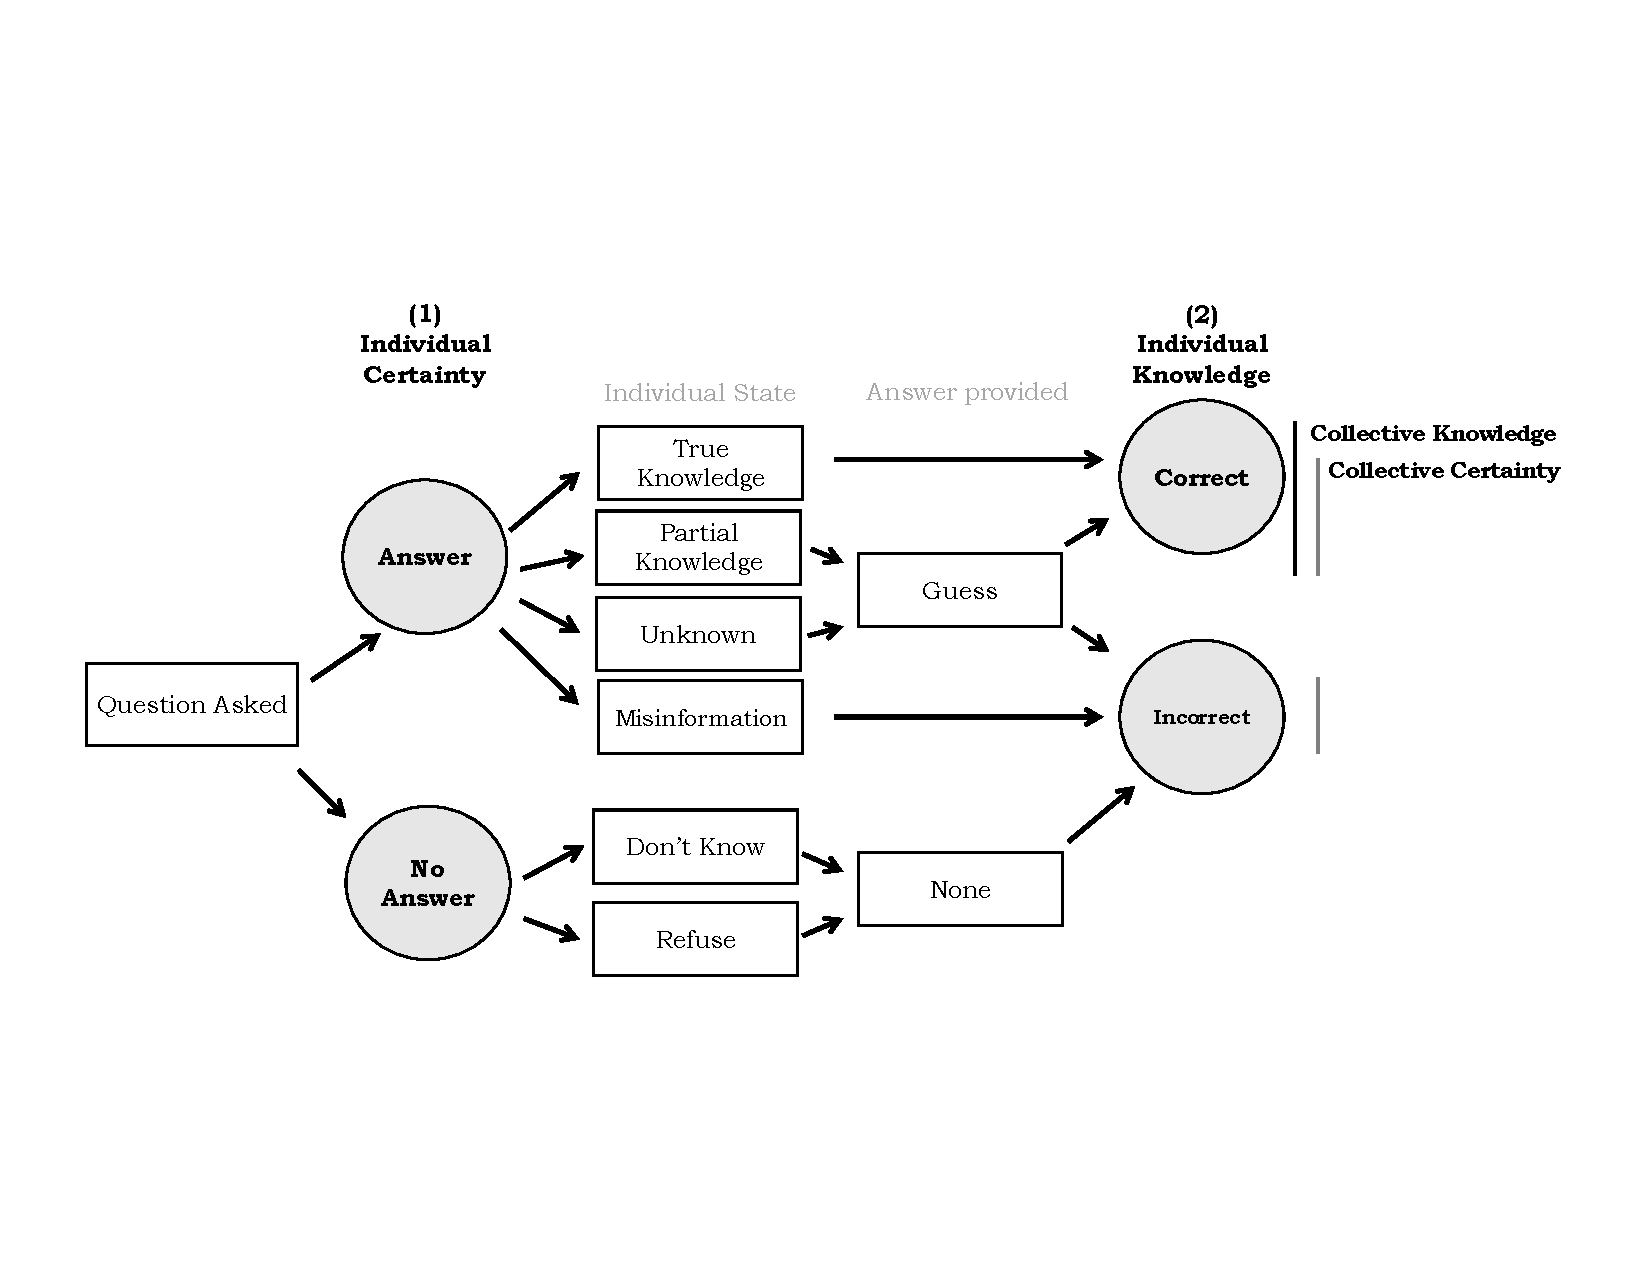
\includegraphics[width=.8\textwidth]{two-step-model-of-knowledge}
  \end{center}
  \caption[A model of responses to knowledge questions]
  {\emph{A model of responses to knowledge questions.}
   My analytical approach conceives of respondents following a two-step decision process when answering factual knowledge questions in surveys. First, the respondent decides if they are sufficiently certain to answer the question or not (a measure of collective certainty when aggregated). Others answer the question either `don't know' or some variation thereof. Conditional on answering, the respondent proceeds to step two, either getting the question correct or incorrect (a measure of misinformation).}
  \label{fig:TwoStepModelOfKnowledge}
\end{figure}

First, I provide a set of descriptive statistics for each question. To evaluate the proportion answering correctly, I estimate the population mean (and standard error) for the binary variable indicating correct answer, within a given demographic group:

 $$ mean_C = \frac{P(y = 1)}{N}. $$

In this model, \emph{N} is the size of the sample responding to that question, and \emph{y = 1} the outcome variable (correct answer). The probability of answering correctly ($P(y = 1)$) is calculated out of all individuals who provided a correct or incorrect answer (including those who respond `don't know'). Hence, the mean value correct for the population for a single knowledge question ($mean_C$) is equal to the survey-weighted probability of getting the knowledge question correct divided by the total number of survey respondents within the group.


%-------%
\subsection{Model}\label{sec:model}

I analyze the likelihood of answering correctly (compared to incorrectly). Because the outcome of interest is dichotomous (correct = 1, incorrect = 0), I analyze the data using logistic regression. Logistic regression is appropriate because it bounds the estimates between 0 and 1. Linear models are ill-suited  because they can yield probability estimates less than 0 or greater than 1. Logistic regression assumes that the distribution of [repeated Bernoulli trials of] the dependent variable (correct answer) follows the binomial distribution. Logistic models link the independent variables to the probability of the dependent variable through the logistic function to estimate parameters. Hence, the probability of the respondent getting knowledge question correct is linked to the set of independent variables through the logistic function

 $$ ln \frac{P(y=1)}{P(y=0)}=x. $$

In this model, $x$ is a vector of independent variables, and $\beta$ is a vector of parameter estimates that measure the effect of the $x$ vector on the log odds that the outcome variable $y = 1$.

%The log-odds that individual i answers question j correctly is represented as a function of individual characteristics:

% $$  ln \frac{P({y_{ij}}=1)}{P({y_{ij}}=0)} =\beta_{0i} + \beta_{edu}Education_i + \beta_{woman}Woman_i + ?_{age}Age_i + \beta_{inc}Income_i + ?_{black}Black_i + $$

%where $\beta_{i0}$ signifies an individual-level random intercept (which can be interpreted as the variation in individuals? knowledge), and the $\beta_j$ coefficients represent group-level random effects, which allow the effect of each variable to vary across questions.


%To assess the role of news consumption and demographic groups in acquiring accurate knowledge about the COVID-19 pandemic, I develop a multiple-step multiple mediator model \citep{Hayes2009}. First, I introduce a baseline model for each knowledge question that includes only demographic characteristics of respondents. Next, I introduce educational attainment as a mediator. Finally, I add the mediator variable of news source.

%Because the analysis uses a survey design, I use an adjusted Wald tests to examine the significance of differences in the coefficients between models \citep{SurveyDatattest}. Wald tests examine the null hypothesis of whether two independent variables, either within or between models, have the same effect on the dependent variable.


%----------------------------------------------------------------------------------------
\section{Results}\label{sec:results}
%----------------------------------------------------------------------------------------

Here I analyze the effect of demographic group membership and news sources on the log odds that people have correct knowledge about questions related to COVID-19. Analyses look at the role of gender, age group, race, family income, and education, in order to explore the role of socioeconomic context and news consumption during the pandemic and knowledge of these questions. 
Summary statistics for each of these demographic factors related to the three knowledge questions are presented in Table~\ref{table:SummaryStats}. This table presents descriptive statistics of the proportion of each group who answered the knowledge questions correctly, adjusted for survey sampling \citep{UCLASurveyDataAnalysis}. For the continuous value of family income, the table presents the income mean value for respondents who answered each question correctly. As the table demonstrates, there are dramatic descriptive disparities among demographic groups in the proportion of the population answering each question correctly.

\begin{table}[htbp]\centering
 % \begin{adjustwidth}{-1cm}{-1cm}
  \caption[Descriptive statistics]
  {\emph{Descriptive Statistics: Proportion of population that answered each question incorrectly and correctly.} Mean and standard deviation (adjusted using survey weights) shown by demographic groups of interest.}
  \label{table:SummaryStats}
{\scriptsize
{\textsymbols
\begin{tabular*}{1\textwidth}{l @{\extracolsep\fill} *{5}{S[table-format=4.6]} @{}}
\hline
                      &\multicolumn{1}{c}{Fauci}  &\multicolumn{1}{c}{State}  &\multicolumn{1}{c}{Antibody}  & \\
                       &\multicolumn{1}{c}{Correct} &\multicolumn{1}{c}{Correct}  &\multicolumn{1}{c}{Correct}  & \\
                        &\multicolumn{1}{c}{Mean / SD}   &\multicolumn{1}{c}{Mean / SD}   &\multicolumn{1}{c}{Mean / SD} &\multicolumn{1}{c}{Observations}    \\
\hline
\multicolumn{5}{l}{\emph{Gender}}                                   \\
\enspace Woman              & .767    & .586    & .695    &   5002  \\
                            & (.007)  & (.008)  & (.008)  &         \\
\enspace Man                & .883    & .632    & .734    &   4238  \\
                            & (.006)  & (.009)  & .008    &         \\
\multicolumn{5}{l}{\emph{Age}}                                      \\
\enspace 18 to 29           & .642    & .539    & .609    &   1006  \\
                            & (.017)  & (.018)  & (.018)  &         \\
\enspace 30 to 49           & .781    & .598    & .715    &   2966  \\
                            & (.009)  & (.011)  & (.010)  &         \\
\enspace 50 to 64           & .855    & .606    & .733    &         \\
                            & (.008)  & (.011)  & (.010)  &         \\
\enspace 65 and over        & .906    & .652    & .731    &   2415  \\
                            & (.007)  & (.011)  & (.011)  &         \\
\emph{Household Inc.} (\$1000)& \\
                            & \\
\multicolumn{5}{l}{\emph{Race}}                                     \\
\enspace White              & .869    & .656    & .789    &   6326  \\
                            & (.005)  & (.007)  & (.006)  &         \\
\enspace Black              & .679    & .465    & .447    &   712   \\
                            & (.020)  & (.022)  & (.022)  &         \\
\enspace Asian              & .825    & .587    & .701    &   270   \\
                            & (.027)  & (.035)  & (.031)  &         \\
\enspace Hispanic           & .694    & .497    & .548    &   1595  \\
                            & (.014)  & (.015)  & (.015)  &         \\
\enspace  Other             & .792    & .540    & .662    &   254   \\
                            & (.029)  & (.036)  & (.034)  &         \\
\enspace      BIPOC         & .719    & .511    & .550    &   1695  \\
                            & (.013)  & (.014)  & (.014)  &         \\
\multicolumn{5}{l}{\emph{Education}}                                \\
\enspace Less than HS       & .466    & .354    & .362    &   234   \\
                            & (.038)  & (.037)  & (.037)  &         \\
\enspace High School        & .621    & .460    & .458    &   1014  \\
                            & (.018)  & (.019)  & (.018)  &         \\
\enspace Some College       & .765    & .577    & .648    &   2752  \\
                            & (.009)  & (.011)  & (.011)  &         \\
\enspace College            & .885    & .641    & .782    &   2748  \\
                            & (.007)  & (.011)  & (.009)  &         \\
\enspace Grad School        & .928    & .692    & .851    &   2489  \\
                            & (.006)  & (.011)  & (.008)  &         \\
\multicolumn{5}{l}{\emph{Source relied most on for news about COVID-19}}  \\
\enspace International News & .827    & .645    & .671    &   369   \\
                            & (.023)  & (.029)  & (.029)  &         \\
\enspace National News      & .912    & .670    & .797    &   2801  \\
                            & (.006)  & (.010)  & (.009)  &         \\
\enspace Local News         & .692    & .483    & .567    &   1262  \\
                            & (.015)  & (.016)  & (.016)  &         \\
\enspace Trump / task force & .854    & .623    & .703    &   1293  \\
                            & (.012)  & (.016)  & (.015)  &         \\
\enspace Biden / campaign   & .367    & .564    & .394    &   16    \\
                            & (.138)  & (.143)  & (.142)  &         \\
\enspace Elected officials  & .864    & .621    & .749    &   849   \\
                            & (.014)  & (.020)  & (.018)  &         \\
\enspace Public Health      & .829    & .633    & .766    &   1842  \\
                            & (.010)  & (.013)  & (.011)  &         \\
\enspace Friends, family    & .402    & .401    & .433    &   204   \\
                            & (.040)  & (.040)  & (.041)  &         \\
\enspace Community          & .480    & .507    & .495    &   30    \\
                            & (.110)  & (.109)  & (.110)  &         \\
\enspace Online forums      & .719    & .608    & .629    &   218   \\
                            & (.035)  & (.038)  & (.037)  &         \\
                       \hline
Observations     &  \\
\hline
\end{tabular*}}}
%\end{adjustwidth} %adjust margins of page for wide table
\end{table}


As Tables~\ref{table:fauciLOs}, \ref{table:stateresponseLOs}, and \ref{table:antibodyLOs} indicate, I analyzed a series of nested models, the first including only the control variables and the final model including all variables. Model 1 in each of Tables~\ref{table:fauciLOs}, \ref{table:stateresponseLOs}, and \ref{table:antibodyLOs} present the basic control models predicting correct knowledge for each of the questions. In this baseline model, age, income, and race are important predictors across all three knowledge questions. Model 2 for each question adds education variables. Finally, Model 3 introduces the variable indicating the source the respondent relied on most for news about COVID-19, allowing us to compare the relative contributions of demographic and information factors in determining correct knowledge. In supplementary analyses, I also investigate interactions of race and news source and of income and news source to see if different groups get different factual knowledge outcomes from consuming different news sources (see Appendix Tables~\ref{table:FauciLOs_appendix}, \ref{table:stateresponseLOs_appendix}, and \ref{table:antibodyLOs_appendix}).


%-------%
% MODELS

%-FAUCI-%
%\item ``Do you happen to know who Anthony Fauci is?'' (Correct answer is ``An infectious disease expert and government health adviser.q)'
\begin{table}[htbp]\centering
  %\begin{adjustwidth}{-1cm}{-1cm}
  \caption[Predicting Knowledge of Fauci: Logistic regressions estimating correct
  knowledge that Anthony Fauci is an infectious disease expert and government
  advisor conditional on demographic and media predictors.]
  {\emph{Predicting Knowledge of Fauci: Logistic regressions estimating correct
  knowledge that Anthony Fauci is an infectious disease expert and government
  advisor conditional on demographic and media predictors. Log odds (and
  linearized standard errors) for each model.}}
  \label{table:fauciLOs}
{\footnotesize
{\textsymbols
\begin{tabular*}{1\textwidth}{l @{\extracolsep\fill} *{5}{S[table-format=4.6]} @{}}
\hline
                  &\multicolumn{1}{c}{(1)}  &\multicolumn{1}{c}{(2)}  &\multicolumn{1}{c}{(3)}  &\multicolumn{1}{c}{(4)}  \\
                  &\multicolumn{1}{c}{Baseline model}  &\multicolumn{1}{c}{Add education} &\multicolumn{1}{c}{Add news source} &\multicolumn{1}{c}{News collapsed}  \\
                  &\multicolumn{1}{c}{$\beta$ / SE}  &\multicolumn{1}{c}{$\beta$ / SE}  &\multicolumn{1}{c}{$\beta$ / SE}  &\multicolumn{1}{c}{$\beta$ / SE}    \\
\hline
\multicolumn{1}{l}{\emph{Gender (woman)}}
                      &      -0.708\sym{***}&      -0.721\sym{***}&      -0.709\sym{***}&      -0.717\sym{***}\\
                      &     (0.073)         &     (0.076)         &     (0.080)         &     (0.080)         \\
\multicolumn{3}{l}{\emph{Age} (Comparison: 18-29)}                &                     &                     \\
\enspace 30 to 49     &       0.543\sym{***}&       0.538\sym{***}&       0.560\sym{***}&       0.540\sym{***}\\
                      &     (0.101)         &     (0.107)         &     (0.112)         &     (0.112)         \\
\enspace 50 to 64     &       1.006\sym{***}&       1.179\sym{***}&       1.095\sym{***}&       1.080\sym{***}\\
                      &     (0.107)         &     (0.114)         &     (0.121)         &     (0.121)         \\
\enspace 65 and over  &       1.350\sym{***}&       1.455\sym{***}&       1.335\sym{***}&       1.305\sym{***}\\
                      &     (0.122)         &     (0.128)         &     (0.136)         &     (0.135)         \\
\multicolumn{1}{l}{\emph{Ln(Household Income)}}
                      &      0.236\sym{***} &      0.154\sym{***} &      0.148\sym{***} &      0.150\sym{***} \\
                      &     (0.026)         &     (0.022)         &     (0.023)         &     (0.023)         \\
\multicolumn{3}{l}{\emph{Race} (Comparison: Non-Hispanic White)}  &                     &                     \\
\enspace Black        &     -0.821\sym{***} &     -0.754\sym{***} &     -0.663\sym{***} &     -0.678\sym{***} \\
                      &     (0.114)         &     (0.117)         &     (0.130)         &     (0.128)         \\
\enspace Asian        &      -0.158         &      -0.449\sym{*}  &      -0.455\sym{*}  &      -0.457\sym{*}  \\
                      &     (0.208)         &     (0.215)         &     (0.212)         &     (0.221)         \\
\enspace Hispanic     &    -0.708\sym{***}  &     -0.536\sym{***} &     -0.519\sym{***} &     -0.542\sym{***} \\
                      &     (0.084)         &     (0.090)         &     (0.094)         &     (0.094)         \\
\enspace Other/mixed  &      -0.279         &      -0.110         &      -0.143         &      -0.142         \\
                      &     (0.188)         &     (0.194)         &     (0.198)         &     (0.196)         \\
\multicolumn{3}{l}{\emph{Education} (Comparison: High School)}    &                     &                     \\
\enspace Less than HS &                     &      -0.334         &      -0.437\sym{*}  &      -0.442\sym{*}  \\
                      &                     &     (0.199)         &     (0.221)         &     (0.218)         \\
\enspace Some College &                     &       0.690\sym{***}&       0.560\sym{***}&       0.581\sym{***}\\
                      &                     &     (0.102)         &     (0.109)         &     (0.108)         \\
\enspace College      &                     &       1.555\sym{***}&       1.425\sym{***}&       1.432\sym{***}\\
                      &                     &     (0.115)         &     (0.124)         &     (0.123)         \\
\enspace Grad School  &                     &       1.865\sym{***}&       1.641\sym{***}&       1.662\sym{***}\\
                      &                     &     (0.131)         &     (0.138)         &     (0.137)         \\
\multicolumn{5}{l}{\emph{Source relied most on for news about COVID-19} (Comparison: National  News)}         \\
\enspace International News&                &                     &      -0.612\sym{**} &                     \\
                      &                     &                     &     (0.210)         &                     \\
\enspace Local News   &                     &                     &      -1.072\sym{***}&                     \\
                      &                     &                     &     (0.119)         &                     \\
\multicolumn{2}{l}{\enspace Trump / COVID task force}&            &      -0.587\sym{***}&                     \\
                      &                     &                     &     (0.128)         &                     \\
\multicolumn{2}{l}{\enspace Biden and his campaign} &             &    -2.378\sym{**}   &                     \\
                      &                     &                     &     (0.759)         &                     \\
\multicolumn{3}{l}{\enspace State and local elected officials}    &      -0.314\sym{*}  &                     \\
                      &                     &                     &     (0.151)         &                     \\
\multicolumn{3}{l}{\enspace Public health organizations and officials} & -0.684\sym{***}&                     \\
                      &                     &                     &     (0.113)         &                     \\
\multicolumn{2}{l}{\enspace Friends, family and neighbors}  &     &      -2.349\sym{***}&                     \\
                      &                     &                     &     (0.199)         &                     \\
\multicolumn{3}{l}{\enspace Community or neighborhood newsletter or Listserv} &  -1.536\sym{**} &             \\
                      &                     &                     &     (0.467)         &                     \\
\multicolumn{3}{l}{\enspace Online forums or discussion groups}   &   -1.157\sym{***}   &                     \\
                      &                     &                     &     (0.213)         &                     \\
\multicolumn{5}{l}{\emph{Source relied most on for news about COVID-19 (Collapsed)} (Comparison: National \& International News)}   \\
\enspace Local news   &                     &                     &                     &      -0.977\sym{***}\\
                      &                     &                     &                     &     (0.114)         \\
\enspace Politicians  &                     &                     &                     &      -0.413\sym{***}\\
                      &                     &                     &                     &     (0.108)         \\
\enspace Public Health&                     &                     &                     &      -0.596\sym{***}\\
                      &                     &                     &                     &       (0.109)       \\
\enspace Informal     &                     &                     &                     &      -1.652\sym{***}\\
                      &                     &                     &                     &     (0.145)         \\
\hline
Observations    &\multicolumn{1}{c}{9079}   &\multicolumn{1}{c}{9069}  &\multicolumn{1}{c}{8763} &\multicolumn{1}{c}{8763}  \\
\hline
\end{tabular*}}}
%\end{adjustwidth} %adjust margins of page for wide table
\end{table}



%-STATE RESPONSE-%
%\item ``As far as you know, how did states in the U.S. respond during the coronavirus outbreak?''" (Correct answer is ``Some states in the U.S. have not had a statewide stay-at-home order.'')
 \begin{table}[htbp]\centering
  %\begin{adjustwidth}{-1cm}{-1cm}
  \caption[Predicting Knowledge of state COVID-19 response: Logistic regressions
  estimating correct knowledge that some states in the U.S. did not have a
  statewide stay-at-home order.]
  {\emph{Predicting Knowledge of state COVID-19 response: Logistic regressions
  estimating correct knowledge that some states in the U.S. did not have a
  statewide stay-at-home order. Log odds (and linearized standard errors) for
  each model.}}
  \label{table:stateresponseLOs}
{\footnotesize
{\textsymbols
\begin{tabular*}{1\textwidth}{l @{\extracolsep\fill} *{5}{S[table-format=4.6]} @{}}
\hline
                      &\multicolumn{1}{c}{(1)}  &\multicolumn{1}{c}{(2)}  &\multicolumn{1}{c}{(3)}  &\multicolumn{1}{c}{(4)}  \\
                      &\multicolumn{1}{c}{Baseline model}  &\multicolumn{1}{c}{Add education} &\multicolumn{1}{c}{Add news source} &\multicolumn{1}{c}{News collapsed}  \\
                      &\multicolumn{1}{c}{$\beta$ / SE}  &\multicolumn{1}{c}{$\beta$ / SE}  &\multicolumn{1}{c}{$\beta$ / SE}  &\multicolumn{1}{c}{$\beta$ / SE}    \\
\hline
\multicolumn{1}{l}{\emph{Gender (woman)}}
                      &      -0.109\sym{*}  &      -0.102         &      -0.070         &      -0.077         \\
                      &     (0.052)         &     (0.052)         &     (0.054)         &     (0.053)         \\
\multicolumn{3}{l}{\emph{Age} (Comparison: 18-29)}                &                     &                    \\
\enspace 30 to 49     &       0.112         &       0.096         &       0.127         &       0.122         \\
                      &     (0.090)         &     (0.090)         &     (0.094)         &     (0.093)         \\
\enspace 50 to 64     &       0.100         &       0.130         &       0.127         &       0.125         \\
                      &     (0.091)         &     (0.091)         &     (0.096)         &     (0.095)         \\
\enspace 65 and over  &       0.217\sym{*}  &       0.212\sym{*}  &       0.200\sym{*}  &       0.198\sym{*}  \\
                      &     (0.094)         &     (0.095)         &     (0.100)         &     (0.100)         \\
\multicolumn{1}{l}{\emph{Ln(Household Income)}}
                      & 0.138\sym{***}      &       0.089\sym{***}&       0.078\sym{***}&       0.078\sym{***}\\
                      &     (0.021)         &     (0.019)         &     (0.019)         &     (0.019)         \\
\multicolumn{3}{l}{\emph{Race} (Comparison: Non-Hispanic White)}  &                     &                     \\
\enspace Black        &      -0.647\sym{***}&      -0.619\sym{***}&      -0.620\sym{***}&    -0.614\sym{***}  \\
                      &     (0.096)         &     (0.096)         &     (0.100)         &     (0.100)         \\
\enspace Asian        &      -0.290\sym{*}  &      -0.384\sym{**} &      -0.413\sym{**} &      -0.401\sym{**} \\
                      &     (0.148)         &     (0.149)         &     (0.154)         &     (0.154)         \\
\enspace Hispanic     &      -0.526\sym{***}&      -0.459\sym{***}&      -0.433\sym{***}&      -0.436\sym{***}\\
                      &     (0.070)         &     (0.071)         &     (0.073)         &     (0.073)         \\
\enspace Other/mixed  &      -0.421\sym{**} &      -0.390\sym{**} &      -0.394\sym{*}  &      -0.393\sym{*}  \\
                      &     (0.150)         &     (0.150)         &     (0.155)         &     (0.153)         \\
\multicolumn{3}{l}{\emph{Education} (Comparison: High School)}    &                     &                     \\
\enspace Less than HS &                     &      -0.222         &      -0.234         &      -0.230         \\
                      &                     &     (0.182)         &     (0.187)         &     (0.187)         \\
\enspace Some College &                     &       0.405\sym{***}&       0.342\sym{***}&       0.350\sym{***}\\
                      &                     &     (0.088)         &     (0.091)         &     (0.091)         \\
\enspace College      &                     &       0.614\sym{***}&       0.529\sym{***}&       0.535\sym{***}\\
                      &                     &     (0.090)         &     (0.093)         &     (0.093)         \\
\enspace Grad School  &                     &       0.789\sym{***}&       0.662\sym{***}&       0.673\sym{***}\\
                      &                     &     (0.093)         &     (0.097)         &     (0.097)         \\
\multicolumn{5}{l}{\emph{Source relied most on for news about COVID-19} (Comparison: National  News)}         \\
\enspace International News&                &                     &      -0.143         &                     \\
                      &                     &                     &     (0.139)         &                     \\
\enspace Local News   &                     &                     &     -0.539\sym{***} &                     \\
                      &                     &                     &     (0.083)         &                     \\
\multicolumn{2}{l}{\enspace Trump / COVID task force} &           &      -0.166         &                     \\
                      &                     &                     &     (0.086)         &                     \\
\multicolumn{2}{l}{\enspace Biden and his campaign} &             &       0.079         &                     \\
                      &                     &                     &     (0.586)         &                     \\
\multicolumn{3}{l}{\enspace State and local elected officials}    &      -0.169         &                     \\
                      &                     &                     &     (0.097)         &                     \\
\multicolumn{3}{l}{\enspace Public health organizations and officials} &      -0.135    &                     \\
                      &                     &                     &     (0.076)         &                     \\
\multicolumn{2}{l}{\enspace Friends, family and neighbors}  &     &    -0.868\sym{***}  &                     \\
                      &                     &                     &     (0.187)         &                     \\
\multicolumn{3}{l}{\enspace Community or neighborhood newsletter or Listserv} &  -0.218 &                     \\
                      &                     &                     &     (0.475)         &                     \\
\multicolumn{3}{l}{\enspace Online forums or discussion groups}   &      -0.163         &                     \\
                      &                     &                     &     (0.173)         &                     \\
\multicolumn{5}{l}{\emph{Source relied most on for news about COVID-19 (Collapsed)} (Comparison: National \& International News)}   \\
\enspace Local news   &                     &                     &                     &      -0.519\sym{***}\\
                      &                     &                     &                     &     (0.081)         \\
\enspace Politicians  &                     &                     &                     &      -0.147\sym{*}  \\
                      &                     &                     &                     &     (0.071)         \\
\enspace Public Health &                    &                     &                     &      -0.117         \\
                      &                     &                     &                     &     (0.074)         \\
\enspace Informal     &                     &                     &                     &      -0.465\sym{***}\\
                      &                     &                     &                     &     (0.126)         \\
\hline
\end{tabular*}}}
%\end{adjustwidth} %adjust margins of page for wide table
\end{table}


%-ANTIBODY TESTS-%
%\item ``As far as you know, are antibody tests for the coronavirus (also known as serology tests) intended to detect?'' (Correct answer is ``A previous infection'')
 \begin{table}[htbp]\centering
  %\begin{adjustwidth}{-1cm}{-1cm}
  \caption[Predicting Knowledge of Antibody tests: Logistic regressions estimating
  correct knowledge that antibody tests for the coronavirus (also known as
  serology tests) are intended to detect a previous infection.]
  {\emph{Predicting Knowledge of Antibody tests: Logistic regressions estimating
  correct knowledge that antibody tests for the coronavirus (also known as
  serology tests) are intended to detect a previous infection. Log odds (and
  linearized standard errors) for each model.}}
  \label{table:antibodyLOs}
{\footnotesize
{\textsymbols
\begin{tabular*}{1\textwidth}{l @{\extracolsep\fill} *{5}{S[table-format=4.6]} @{}}
\hline
                      &\multicolumn{1}{c}{(1)}  &\multicolumn{1}{c}{(2)}  &\multicolumn{1}{c}{(3)}  &\multicolumn{1}{c}{(4)}  \\
                      &\multicolumn{1}{c}{Baseline model}  &\multicolumn{1}{c}{Add education} &\multicolumn{1}{c}{Add news source} &\multicolumn{1}{c}{News collapsed}  \\
                      &\multicolumn{1}{c}{$\beta$ / SE}  &\multicolumn{1}{c}{$\beta$ / SE}  &\multicolumn{1}{c}{$\beta$ / SE}  &\multicolumn{1}{c}{$\beta$ / SE}    \\
\hline
\multicolumn{1}{l}{\emph{Gender (woman)}}
                      &      -0.053         &      -0.029         &      -0.019         &      -0.017         \\
                      &     (0.059)         &     (0.060)         &     (0.063)         &     (0.062)         \\
\multicolumn{3}{l}{\emph{Age} (Comparison: 18-29)}                &                     &                    \\
\enspace 30 to 49     &       0.269\sym{**} &       0.257\sym{*}  &       0.255\sym{*}  &       0.245\sym{*}  \\
                      &     (0.096)         &     (0.100)         &     (0.104)         &     (0.104)         \\
\enspace 50 to 64     &       0.262\sym{**} &       0.352\sym{***}&       0.282\sym{**} &       0.281\sym{**} \\
                      &     (0.100)         &     (0.102)         &     (0.107)         &     (0.107)         \\
\enspace 65 and over  &       0.105         &       0.102         &       0.032         &       0.027         \\
                      &     (0.102)         &     (0.106)         &     (0.112)         &     (0.112)         \\
\multicolumn{1}{l}{\emph{Ln(Household Income)}}
                      &       0.311\sym{***}&       0.201\sym{***}&       0.212\sym{***}&       0.213\sym{***}\\
                      &     (0.042)         &     (0.028)         &     (0.028)         &     (0.029)         \\
\multicolumn{3}{l}{\emph{Race} (Comparison: Non-Hispanic White)}  &                     &                     \\
\enspace Black        &      -1.377\sym{***}&      -1.408\sym{***}&      -1.435\sym{***}&      -1.423\sym{***}\\
                      &     (0.099)         &     (0.103)         &     (0.108)         &     (0.107)         \\
\enspace Asian        &      -0.521\sym{***}&      -0.776\sym{***}&      -0.843\sym{***}&      -0.854\sym{***}\\
                      &     (0.158)         &     (0.160)         &     (0.166)         &     (0.167)         \\
\enspace Hispanic     &      -0.972\sym{***}&      -0.894\sym{***}&      -0.893\sym{***}&      -0.908\sym{***}\\
                      &     (0.073)         &     (0.076)         &     (0.078)         &     (0.078)         \\
\enspace Other/mixed  &      -0.572\sym{***}&      -0.489\sym{**} &      -0.528\sym{**} &      -0.526\sym{**} \\
                      &     (0.162)         &     (0.163)         &     (0.168)         &     (0.167)         \\
\multicolumn{3}{l}{\emph{Education} (Comparison: High School)}    &                     &                     \\
\enspace Less than HS &                     &      -0.006         &      -0.096         &      -0.096         \\
                      &                     &     (0.195)         &     (0.205)         &     (0.203)         \\
\enspace Some College &                     &       0.741\sym{***}&       0.658\sym{***}&       0.668\sym{***}\\
                      &                     &     (0.092)         &     (0.095)         &     (0.095)         \\
\enspace College      &                     &       1.284\sym{***}&       1.165\sym{***}&       1.173\sym{***}\\
                      &                     &     (0.098)         &     (0.103)         &     (0.102)         \\
\enspace Grad School  &                     &       1.673\sym{***}&       1.483\sym{***}&       1.495\sym{***}\\
                      &                     &     (0.107)         &     (0.112)         &     (0.111)         \\
\multicolumn{5}{l}{\emph{Source relied most on for news about COVID-19} (Comparison: National  News)}         \\
\enspace International News&                &                     &    -0.591\sym{***}  &                     \\
                      &                     &                     &     (0.155)         &                     \\
\enspace Local News   &                     &                     &      -0.768\sym{***}&                     \\
                      &                     &                     &     (0.094)         &                     \\
\multicolumn{2}{l}{\enspace Trump / COVID task force}   &         &      -0.454\sym{***}&                     \\
                      &                     &                     &     (0.098)         &                     \\
\multicolumn{2}{l}{\enspace Biden and his campaign} &             &     -0.967          &                     \\
                      &                     &                     &     (0.573)         &                     \\
\multicolumn{3}{l}{\enspace State and local elected officials}    &      -0.273\sym{*}  &                     \\
                      &                     &                     &     (0.122)         &                     \\
\multicolumn{3}{l}{\enspace Public health organizations and officials} & -0.246\sym{**} &                     \\
                      &                     &                     &     (0.092)         &                     \\
\multicolumn{2}{l}{\enspace Friends, family and neighbors}  &     &      -1.360\sym{***}&                     \\
                      &                     &                     &     (0.187)         &                     \\
\multicolumn{3}{l}{\enspace Community or neighborhood newsletter or Listserv} &  -0.622 &                     \\
                      &                     &                     &     (0.513)         &                     \\
\multicolumn{3}{l}{\enspace Online forums or discussion groups}   &     -0.595\sym{**}  &                     \\
                      &                     &                     &     (0.184)         &                     \\
\multicolumn{5}{l}{\emph{Source relied most on for news about COVID-19 (Collapsed)} (Comparison: National \& International News)}   \\
\enspace Local news   &                     &                     &                     &      -0.686\sym{***}\\
                      &                     &                     &                     &     (0.091)         \\
\enspace Politicians  &                     &                     &                     &      -0.311\sym{***}\\
                      &                     &                     &                     &     (0.083)         \\
\enspace Public Health&                     &                     &                     &      -0.167         \\
                      &                     &                     &                     &     (0.089)         \\
\enspace Informal     &                     &                     &                     &      -0.864\sym{***}\\
                      &                     &                     &                     &     (0.131)         \\
\hline
Observations   &\multicolumn{1}{c}{9079}    &\multicolumn{1}{c}{9069} &\multicolumn{1}{c}{8763} &\multicolumn{1}{c}{8763}  \\
\hline
\end{tabular*}}}
%\end{adjustwidth} %adjust margins of page for wide table
\end{table}




%-------%
\subsection{Gender}\label{sec:gender}

Women are significantly less likely to correctly identify Fauci as an infectious disease expert and government advisor, an effect that does not disappear with later additions of education and news variables. This difference may be attributable to women's tendency to follow political news less than men \citep{Verba1997}. In the baseline Model 1, women are also less likely to correctly answer that some states did not have a stay-at-home order, though this effect is moderate and disappears in later models. There is no significant difference between women and men in correct knowledge of antibody tests, perhaps the most important fact for health outcomes. 

\subsection{Age}

Older age groups are significantly more likely to know that Fauci is an infectious disease expert and government advisor, even controlling for education and primary news source. The older you are, the more likely you are to know who  Fauci is, as well. %need to do test
This held across all models. 
This is not the case with knowledge about statewide stay-at-home orders. Only those in the 65 and over age group were slightly more likely to have correct knowledge of this question, compared to those ages 18 to 29 (p$<$.05 for Model 3 in Table~\ref{table:stateresponseLOs}). Finally, this is in contrast to knowledge about antibody tests. Only those in the middle two age groups, 30 to 49 (p$<$.05) and 50 to 64 (p$<$.01), had more knowledge of the antibody tests, compared to 18- to 29-year-olds. 


%-------%
\subsection{Income}\label{sec:income}

Across all models and questions, family income has a significant effect on how likely people are to be correct about COVID-19 facts. The addition of education into the models (from Model 1 to Model 2 in Tables~\ref{table:fauciLOs}, \ref{table:stateresponseLOs}, and \ref{table:antibodyLOs}) naturally reduces the magnitude of the effect of income on the likelihood of knowing the correct answer, but in no case does it eliminate the effect altogether.

In the full Model 3 in Table~\ref{table:fauciLOs}, each additional 1\% increase in family income increases the log-odds of knowing who Fauci is by 0.148, holding constant gender, age group, race, education, and news source (p$<$.001). 
Each additional 1\% increase in family income significantly increases the log-odds of knowing some states did not have a stay at home order by 0.078 (Model 3 in Table~\ref{table:stateresponseLOs}), all else constant (p$<$.001).
In the effect with the greatest magnitude, each additional 1\% increase in family income significantly increases the odds of knowing that antibody tests are intended to detect previous infection by 23.6\% (p$<$.001). %[(exp(0.212)-1)*\%=] 
Overall, family income has a positive and significant effect on the likelihood of having knowledge of COVID-19 topics in these three different and important areas: governmental, public health, and scientific knowledge.


%-------%
\subsection{Race}\label{sec:race}

All models show a significant effect of the race of the respondent on the likelihood of answering the question correctly. This holds true regardless of whether race is modeled using the pentagon classification (Black, Asian, Hispanic, Other / mixed, and White, as seen in Tables~\ref{table:fauciLOs}, \ref{table:stateresponseLOs}, and \ref{table:antibodyLOs}) or using a binary BIPOC variable (White and non-White, as seen in Appendix Tables~\ref{table:FauciLOs_appendix}, \ref{table:stateresponseLOs_appendix}, and \ref{table:antibodyLOs_appendix}).

There is a significant negative effect of being Black (compared to being white) on the likelihood of knowing the correct answer to all questions. The effect is striking: Black people are about half as likely to know the answer to each question, controlling for age, income, education, and news source (model 3 in tables~\ref{table:fauciLOs}, \ref{table:stateresponseLOs}, and \ref{table:antibodyLOs}). Specifically, being Black decreased the odds of knowing the correct answer about Fauci by a factor of 0.48 ($p<0.001$), %[$e^{?0.66}-1$ =]
decreased the odds of knowing the correct answer about statewide stay-at-home orders by a factor of 0.46 ($p<0.001$), % [$e^{?0.62}-1$ =]
and decreased the odds of knowing the correct answer about antibodies by a factor of 0.76 (p$<$0.001). %[$e^{?1.435}-1$ =]
There are similar negative effects of being Asian and Hispanic, although the magnitudes are not as great.

%-------%
\subsection{Education}\label{sec:education}

These effects of income and race persist when controlling for education (see Models 2 and 3 in Tables~\ref{table:fauciLOs}, \ref{table:stateresponseLOs}, and \ref{table:antibodyLOs}). Furthermore, each additional level of educational attainment significantly increases the odds of answering correctly, except completing High School. Adding in variables for the source of news does somewhat reduce the magnitude of the effect of education, but it does not eliminate the significance of education in any of the models across any of the knowledge questions. Considering that the effect of education holds in models where family income is also controlled, this speaks to the importance of education in acquiring and digesting information in order to attain accurate knowledge about COVID-19.


%-------%
\subsection{News Source}\label{sec:news source}

Next, I added in variables for the news source the respondent relied on most for news about the coronavirus pandemic (see Model 3 in Tables~\ref{table:fauciLOs}, \ref{table:stateresponseLOs}, and \ref{table:antibodyLOs}).

Notably, those who primarily get their news about COVID-19 through national news sources are the most likely to answer all three questions correctly. Respondents who consume their news from any other source (including, surprisingly, public health officials) were significantly less likely to correctly identify Fauci's role, controlling for all other factors. The same held true for correct knowledge about antibody tests. Those who rely primarily on national news for information about COVID-19 were most likely to correctly answer this question, controlling for gender, age, family income, race, and education.

Those who received their information primarily from local news were significantly less likely to know that some states in the U.S. did not have a statewide stay-at-home order, as were those who primarily relied on friends, family, and neighbors for their news. However, those who rely on state and local elected officials or community or neighborhood newsletters or listservs for their information were just as likely as those relying on national news to know that some states did not have statewide orders, all other variables held equal. This is an interesting contrast to those relying on local news; it seems that the particular \emph{form} of local information matters when it comes to having accurate knowledge about nationwide events.

Relying on friends, family, and neighbors for information about COVID-19 was the most consistent predictor of error, with these respondents only between 0.095 and 0.42 times as likely to answer correctly than those relying on national news (holding constant all other factors).

I also derive a collapsed version of the news source variable (Appendix Tables~\ref{table:FauciLOs_appendix}, \ref{table:stateresponseLOs_appendix}, and \ref{table:antibodyLOs_appendix}: Model~3), which I later use to investigate interaction effects. In moving from ten news source categories to five, the substantive nature of the results remains largely unchanged. All variables remain significant in predicting correct answers about Fauci. Where relying on local news and friends, family, and neighbors were significant predictors of knowledge about a stay-at-home order, the collapsed categories of local news and informal networks remain significant, with the new combined category of politicians also becoming significant. Finally, the collapsed predictor category of public health officials and organizations does become non-significant in predicting knowledge of antibodies, but all others remain significant.

%-------%
\subsection{Interactions with News Source}\label{sec:race-news}

I used these collapsed news source categories to test interactions with race and income. First, I tested interactions of binary BIPOC race and news source, using the collapsed news source variable (see Model~4 in Appendix Tables~\ref{table:FauciLOs_appendix}, \ref{table:stateresponseLOs_appendix}, and \ref{table:antibodyLOs_appendix}). Surprisingly, there is only one significant interaction effect here. Being BIPOC and relying on Public Health officials decreases the odds of knowing the correct answer about Fauci by a factor of 0.882 %[exp(0.541-0.666) =]
compared to being White and relying on Public Health officials. For all other news sources, race does not have a differential effect on whether people have correct knowledge about COVID-19.\footnote
    {Technically, the statistically accurate statement is that I cannot prove that the effect of news on racial category is not uniform.}

%Being black and relying on national news, however, decreased the odds of knowing
%the correct answer by a factor of [exp(-0.666) =] 0.514.

% constant BIPOC = 0    Public Health = 0
%          BIPOC = 1    Public Health = 0       LO = ?0.666   baseline odds decreases by a factor exp(?0.666)=.514
%          BIPOC = 0    Public Health = 1       LO = ?0.717   baseline odds decreases by a factor exp(?0.717)=.488
%          BIPOC = 1    Public Health = 1       LO = 0.541

% black and rely on public health: baseline odds decreases by a factor of exp(0.541-0.717-0.666) = 0.431
% white and rely on public health: exp(-0.717)
% black and rely on natl news:     exp(-0.666)

I also tested interactions of income and news source (see Model~5 in Appendix Tables~\ref{table:FauciLOs_appendix}, \ref{table:stateresponseLOs_appendix}, and \ref{table:antibodyLOs_appendix}). The only significant interaction effect in this model is the impact of income on the effect of local news on knowledge of statewide stay-at-home orders. Those with higher family incomes who rely primarily on local news for information about the coronavirus pandemic are more likely than those with lower incomes to extract accurate information about the state responses from that news. There is no detectable differential effect of income on how other news sources influence other types of knowledge. These results are robust to the omission of education variables from the model. 

% constant Inc = 0    Local News = 0
%          Inc = 1    Local News = 0       LO = 0.073
%          Inc = 0    Local News = 1       LO = -2.992   
%          Inc = 1    Local News = 1       LO = 0.227
%additional 1% income and rely on local news: baseline odds decreases by a factor of exp(0.227-) = 

Overall, there are few differential effects of race or income on how new sources influence knowledge of COVID-19. However, two important limitations apply. First, the two significant effects that are present may be the result of chance.\footnote
    {Concerns about these results being significant solely due to chance are particularly apt because these analyses do not control for multiple comparisons or multiple testing \citep{Howell2012}.} 
Furthermore, I cannot determine if the lack of additional significant interactions is indicative of real-world conditions or merely a lack of statistical power to detect interaction effects.


%----------------------------------------------------------------------------------------
\section{Discussion \& Conclusions}\label{sec:conclusion}
%----------------------------------------------------------------------------------------

This paper describes the current state of COVID-19 knowledge in the U.S. as a function of demographic characteristics and news consumption. This makes it a contribution in the style of Mannheim's sociology of knowledge \citep{Mannheim1929,Swidler1994} and the study of demographic inequalities in gender, age, class, and race and ethnicity. 

Individuals face the world with different sets of knowledge, shaped by their social contexts. Some of this knowledge may be correct, and some of it may be incorrect, as we see in the results of this analysis. Misinformation is an important emerging topic in information science and sociology \citep{Metaxa-Kakavouli2017}: How do we come to know what we know? How do we come to be misinformed? Both, often through engagement with news sources and informal sources. Contrary to current popular narratives that news media, search algorithms, and other sources of factual information are pushing users in biased ways that depend on the demographics of the user, this study finds that there are few statistically significant interactions between news source and demographic characteristics. 

However, this does not mean that certain demographic groups do not gravitate toward more or less effective forms of information. My results show that there are clear demographic distinctions in who knows what facts about the coronavirus pandemic. There are also clear descriptive patterns in media consumption between these groups. Education has persistent effects on the likelihood of knowing all of the questions, although its effects do differ among questions focused on governmental  (Fauci), public health (state stay-at-home order), and scientific (antibody tests) knowledge. The results find that both news source and demographic identities are significant predictors of whether or not people answer questions related to COVID-19 correctly. Race has the most consistent and dramatic effect on correct knowledge about antibody tests, even controlling for income, education, and news source. In contrast, news source and income seem to have the most influence on whether respondents knew that Anthony Fauci is an infectious disease expert and government advisor. However, news source does not have much of a \emph{differential} effect on knowledge based on the race or income of the respondent. Put another way, I cannot reject the hypothesis that race and income have similar effects across news sources.

This study documents concrete evidence on different groups' command over different types of information resources, a matter of increasing importance in modern society. It aims to understand how identity categories influence consumption of information, including some vital to health outcomes during COVID-19. Democracy depends on collective decision-making, which in turn depends on trust in institutions and access to reliable information. Once we better understand the ways social contexts shape information consumption and knowledge, we can design better systems to improve information accuracy and dissemination in the media, government, and other sociotechnical institutions. 




%----------------------------------------------------------------------------------------
\section{Data Availability}\label{sec:data-availability}
%----------------------------------------------------------------------------------------

The research described in this paper relies on a publicly available dataset from surveys administered by the Pew Research Center.
In keeping with recommendations on transparent and open social science \citep{Freese2018}, all code used to analyze these data are available at the Open Science Framework project repository at : [redacted for blind review].


%----------------------------------------------------------------------------------------
\section{Acknowledgments}\label{sec:acknowledgments}
%----------------------------------------------------------------------------------------


%----------------------------------------------------------------------------------------
\subsection{Funding}\label{sec:funding}
%-------------------------------------------


%----------------------------------------------------------------------------------------
\newpage
\section{Appendix}
%----------------------------------------------------------------------------------------
%-FOLLOW CLOSELY-%
\input{followClosely}

%-FAUCI-%
%\item ``Do you happen to know who Anthony Fauci is?'' (Correct answer is ``An infectious disease expert and government health adviser.q)'
\begin{table}[htbp]\centering
  \begin{adjustwidth}{-1cm}{-1cm}
  \caption[Predicting Knowledge of Fauci: Logistic regressions estimating correct
  knowledge that Anthony Fauci is an infectious disease expert and government
  advisor conditional on demographic and media predictors.]
  {\emph{Predicting Knowledge of Fauci: Logistic regressions estimating correct
  knowledge that Anthony Fauci is an infectious disease expert and government
  advisor conditional on demographic and media predictors. Log odds (and
  linearized standard errors) for each model.}}
  \label{table:FauciLOs_appendix}
   {\footnotesize
   {\textsymbols
\begin{tabular*}{1.2\textwidth}{l @{\extracolsep\fill} *{6}{S[table-format=4.6]} @{}}
\hline
&\multicolumn{1}{c}{(1)}&\multicolumn{1}{c}{(2)}&\multicolumn{1}{c}{(3)}&\multicolumn{1}{c}{(4)}&\multicolumn{1}{c}{(5)}\\
&\multicolumn{1}{c}{Baseline model} &\multicolumn{1}{c}{Add education} &\multicolumn{1}{c}{Add news source} &\multicolumn{1}{c}{BIPOC interactions} &\multicolumn{1}{c}{Income interactions} \\
&\multicolumn{1}{c}{$\beta$ / SE}  &\multicolumn{1}{c}{$\beta$ / SE}  &\multicolumn{1}{c}{$\beta$ / SE}  &\multicolumn{1}{c}{$\beta$ / SE} &\multicolumn{1}{c}{$\beta$ / SE}     \\
\hline
\multicolumn{1}{l}{\emph{Gender (woman)}}
                      &     -0.743\sym{***} &    -0.739\sym{***}  &    -0.732\sym{***}  &    -0.728\sym{***}  &    -0.732\sym{***}  \\
                      &     (0.074)         &     (0.076)         &     (0.080)         &     (0.080)         &   (0.080)           \\
\multicolumn{3}{l}{\emph{Age} (Comparison: 18-29)}                &                     &                     &                     \\
\enspace 30 to 49     &      0.552\sym{***} &      0.546\sym{***} &      0.554\sym{***} &      0.551\sym{***} &     0.551\sym{***}  \\
                      &     (0.100)         &     (0.107)         &     (0.112)         &     (0.112)         &    (0.112)          \\
\enspace 50 to 64     &      1.043\sym{***} &      1.210\sym{***} &      1.127\sym{***} &      1.123\sym{***} &     1.122\sym{***}  \\
                      &     (0.108)         &     (0.114)         &     (0.121)         &     (0.121)         &      (0.121)        \\
\enspace 65 and over  &      1.423\sym{***} &     1.523\sym{***}  &      1.374\sym{***} &      1.368\sym{***} &     1.371\sym{***}  \\
                      &     (0.121)         &     (0.127)         &     (0.134)         &     (0.134)         &     (0.134)         \\
\multicolumn{1}{l}{\emph{Ln(Household Income)}}
                      &   0.256\sym{***}    &      0.166\sym{***} &      0.163\sym{***} &      0.163\sym{***} &      0.195\sym{***} \\
                      &     (0.027)         &     (0.023)         &     (0.024)         &     (0.023)         &       (0.037)       \\
\multicolumn{1}{l}{\emph{BIPOC (Non-White)}}
                      &   -0.508\sym{***}   &    -0.444\sym{***}  &    -0.426\sym{***}  &  -0.666\sym{***}    &     -0.426\sym{***} \\
                      &     (0.081)         &     (0.084)         &     (0.088)         &    (0.162)          &     (0.088)         \\
\multicolumn{3}{l}{\emph{Education} (Comparison: High School)}    &                     &                     &                     \\
\enspace Less than HS &                     &      -0.442\sym{*}  &      -0.519\sym{*}  &      -0.517\sym{*}  &     -0.517\sym{*}   \\
                      &                     &     (0.205)         &     (0.223)         &     (0.222)         &       (0.223)       \\
\enspace Some College &                     &       0.684\sym{***}&      0.571\sym{***} &      0.566\sym{***} &     0.572\sym{***}  \\
                      &                     &     (0.102)         &     (0.108)         &     (0.108)         &      (0.108)        \\
\enspace College      &                     &       1.565\sym{***}&      1.438\sym{***} &      1.431\sym{***} &     1.435\sym{***}  \\
                      &                     &     (0.115)         &     (0.123)         &     (0.123)         &     (0.123)         \\
\enspace Grad School  &                     &       1.871\sym{***}&      1.655\sym{***} &      1.646\sym{***} &   1.655\sym{***}    \\
                      &                     &     (0.130)         &     (0.137)         &     (0.137)         &     (0.137)         \\
\multicolumn{5}{l}{\emph{Source relied most on for news about COVID-19} (Comparison: National \& International News)}  &            \\
\enspace Local News   &                     &                     &     -1.022\sym{***} &     -1.107\sym{***} &    -0.632           \\
                      &                     &                     &     (0.115)         &     (0.136)         &   (0.824)           \\
\enspace Politicians  &                     &                     &     -0.393\sym{***} &     -0.442\sym{***} &   0.186             \\
                      &                     &                     &     (0.109)         &     (0.127)         &   (0.586)           \\
\enspace Public Health &                    &                     &     -0.580\sym{***} &     -0.717\sym{***} &   -0.094            \\
                      &                     &                     &     (0.110)         &     (0.129)         &     (0.615)         \\
\enspace Informal Sources &                 &                     &     -1.646\sym{***} &     -1.782\sym{***} &     -1.022          \\
                      &                     &                     &     (0.146)         &     (0.167)         &   (1.335)           \\
\multicolumn{3}{l}{\emph{Interactions}}                           &                     &                     &                     \\
\enspace BIPOC * Local News &               &                     &                     &       0.279         &                     \\
                      &                     &                     &                     &     (0.250)         &                     \\
\enspace BIPOC * Politicians   &            &                     &                     &       0.103         &                     \\
                      &                     &                     &                     &     (0.254)         &                     \\
\enspace BIPOC * Public Health &            &                     &                     &       0.541\sym{*}  &                     \\
                      &                     &                     &                     &     (0.247)         &                     \\
\enspace BIPOC * Informal &                 &                     &                     &       0.472         &                     \\
                      &                     &                     &                     &     (0.330)         &                     \\
\enspace Income * Local News &              &                     &                     &                     &   -0.037            \\
                      &                     &                     &                     &                     &   (0.077)           \\
\enspace Income * Politicians &             &                     &                     &                     &   -0.055            \\
                      &                     &                     &                     &                     &   (0.054)           \\
\enspace Income * Public Health &           &                     &                     &                     &    -0.046           \\
                      &                     &                     &                     &                     &   (0.056)           \\
\enspace Income * Informal &                &                     &                     &                     &  -0.059             \\
                      &                     &                     &                     &                     &   (0.124)           \\
\hline
Observations          & \multicolumn{1}{c}{9008} & \multicolumn{1}{c}{8998} & \multicolumn{1}{c}{8697} & \multicolumn{1}{c}{8697} & \multicolumn{1}{c}{8697} \\
\hline
\end{tabular*}}}
\end{adjustwidth} %adjust margins of page for wide table
\end{table}



%-STATE RESPONSE-%
%\item ``As far as you know, how did states in the U.S. respond during the coronavirus outbreak?''" (Correct answer is ``Some states in the U.S. have not had a statewide stay-at-home order.'')
 \begin{table}[htbp]\centering
  \begin{adjustwidth}{-1cm}{-1cm}
  \caption[Predicting Knowledge of state COVID-19 response: Logistic regressions
  estimating correct knowledge that some states in the U.S. did not have a
  statewide stay-at-home order.]
  {\emph{Predicting Knowledge of state COVID-19 response: Logistic regressions
  estimating correct knowledge that some states in the U.S. did not have a
  statewide stay-at-home order. Log odds (and linearized standard errors) for
  each model.}}
  \label{table:stateresponseLOs_appendix}
{\footnotesize
{\textsymbols
\begin{tabular*}{1.2\textwidth}{l @{\extracolsep\fill} *{6}{S[table-format=4.6]} @{}}
\hline
&\multicolumn{1}{c}{(1)}&\multicolumn{1}{c}{(2)}&\multicolumn{1}{c}{(3)}&\multicolumn{1}{c}{(4)}&\multicolumn{1}{c}{(5)}\\
&\multicolumn{1}{c}{Baseline model} &\multicolumn{1}{c}{Add education} &\multicolumn{1}{c}{Add news source} &\multicolumn{1}{c}{BIPOC interactions} &\multicolumn{1}{c}{Income interactions} \\
&\multicolumn{1}{c}{$\beta$ / SE}  &\multicolumn{1}{c}{$\beta$ / SE}  &\multicolumn{1}{c}{$\beta$ / SE}  &\multicolumn{1}{c}{$\beta$ / SE} &\multicolumn{1}{c}{$\beta$ / SE}     \\
\hline
\multicolumn{1}{l}{\emph{Gender (woman)}}
                      &      -0.116\sym{*}  &      -0.104\sym{*}  &      -0.077         &      -0.078         &   -0.073            \\
                      &     (0.052)         &     (0.052)         &     (0.053)         &     (0.053)         &    (0.053)          \\
\multicolumn{3}{l}{\emph{Age} (Comparison: 18-29)}                &                     &                     &                     \\
\enspace 30 to 49     &       0.126         &       0.108         &       0.135         &       0.140         &     0.135           \\
                      &     (0.089)         &     (0.090)         &     (0.093)         &     (0.093)         &     (0.093)         \\
\enspace 50 to 64     &       0.135         &       0.162         &       0.155         &       0.161         &     0.158           \\
                      &     (0.090)         &     (0.090)         &     (0.094)         &     (0.094)         &    (0.095)          \\
\enspace 65 and over  &       0.289\sym{**} &       0.279\sym{**} &       0.258\sym{**} &       0.262\sym{**} &    0.261\sym{**}    \\
                      &     (0.093)         &     (0.093)         &     (0.098)         &     (0.098)         &    (0.098)          \\
\multicolumn{1}{l}{\emph{Ln(Household Income)}}
                      &      0.157\sym{***} &      0.102\sym{***} &      0.092\sym{***} &      0.092\sym{***} &    0.073\sym{*}     \\
                      &     (0.022)         &     (0.020)         &     (0.019)         &     (0.019)         &    (0.032)          \\
\multicolumn{1}{l}{\emph{BIPOC (Non-White)}}
                      &     -0.396\sym{***} &     -0.372\sym{***} &     -0.371\sym{***} & -0.386\sym{***}     &   -0.366\sym{***}   \\
                      &     (0.065)         &     (0.066)         &     (0.068)         &       (0.110)       &     (0.068)         \\
\multicolumn{3}{l}{\emph{Education} (Comparison: High School)}    &                     &                     &                     \\
\enspace Less than HS &                     &      -0.331         &      -0.315         &      -0.317         &      -0.309         \\
                      &                     &     (0.182)         &     (0.187)         &     (0.187)         &     (0.189)         \\
\enspace Some College &                     &      0.404\sym{***} &      0.350\sym{***} &      0.348\sym{***} &     0.333\sym{***}  \\
                      &                     &     (0.088)         &     (0.091)         &     (0.091)         &    (0.092)          \\
\enspace College      &                     &      0.621\sym{***} &      0.539\sym{***} &      0.538\sym{***} &   0.519\sym{***}    \\
                      &                     &     (0.090)         &     (0.094)         &     (0.094)         &   (0.094)           \\
\enspace Grad School  &                     &      0.796\sym{***} &      0.674\sym{***} &      0.672\sym{***} &    0.662\sym{***}   \\
                      &                     &     (0.093)         &     (0.097)         &     (0.097)         &    (0.098)          \\
\multicolumn{6}{l}{\emph{Source relied most on for news about COVID-19} (Comparison: National \& International News)}               \\
\enspace Local News   &                     &                     &   -0.544\sym{***}   &     -0.500\sym{***} &  -2.992\sym{***}    \\
                      &                     &                     &     (0.081)         &     (0.093)         &   (0.855)           \\
\enspace Politicians  &                     &                     &      -0.129         &      -0.146         &   -0.062            \\
                      &                     &                     &     (0.071)         &     (0.077)         &    (0.539)          \\
\enspace Public Health &                    &                     &      -0.107         &      -0.105         &     0.120           \\
                      &                     &                     &     (0.074)         &     (0.083)         &    (0.535)          \\
\enspace Informal Sources &                 &                     &     -0.461\sym{***} &     -0.568\sym{***} &     -0.303          \\
                      &                     &                     &     (0.125)         &     (0.143)         &    (0.809)          \\
\multicolumn{3}{l}{\emph{Interactions}}                           &                     &                     &                     \\
\enspace BIPOC * Local News &               &                     &                     &      -0.191         &                     \\
                      &                     &                     &                     &     (0.191)         &                     \\
\enspace BIPOC * Politicians &              &                     &                     &       0.121         &                     \\
                      &                     &                     &                     &     (0.192)         &                     \\
\enspace BIPOC * Public Health &            &                     &                     &      -0.010         &                     \\
                      &                     &                     &                     &     (0.184)         &                     \\
\enspace BIPOC * Informal &                 &                     &                     &       0.407         &                     \\
                      &                     &                     &                     &     (0.279)         &                     \\
\enspace Income * Local News &              &                     &                     &                     &   0.227\sym{**}     \\
                      &                     &                     &                     &                     &    (0.078)          \\
\enspace Income * Politicians &             &                     &                     &                     &    -0.006           \\
                      &                     &                     &                     &                     &   (0.049)           \\
\enspace Income * Public Health &           &                     &                     &                     &     -0.020          \\
                      &                     &                     &                     &                     &    (0.048)          \\
\enspace Income * Informal &                &                     &                     &                     &     -0.016          \\
                      &                     &                     &                     &                     &      (0.075)        \\
\hline
Observations        & \multicolumn{1}{c}{9008} &\multicolumn{1}{c}{8998} &\multicolumn{1}{c}{8697}  &\multicolumn{1}{c}{8697} &\multicolumn{1}{c}{8697}   \\
\hline
\end{tabular*}}}
\end{adjustwidth} %adjust margins of page for wide table
\end{table}


%-ANTIBODY TESTS-%
%\item ``As far as you know, are antibody tests for the coronavirus (also known as serology tests) intended to detect?'' (Correct answer is ``A previous infection'')
 \begin{table}[htbp]\centering
\begin{adjustwidth}{-1cm}{-1cm}
   \caption[Predicting Knowledge of Antibody tests: Logistic regressions estimating
   correct knowledge that antibody tests for the coronavirus (also known as
   serology tests) are intended to detect a previous infection.]
   {\emph{Predicting Knowledge of Antibody tests: Logistic regressions estimating
   correct knowledge that antibody tests for the coronavirus (also known as
   serology tests) are intended to detect a previous infection. Log odds (and
   linearized standard errors) for each model.}}
   \label{table:antibodyLOs_appendix}
   {\footnotesize
   {\textsymbols
   \begin{tabular*}{1.2\textwidth}{l @{\extracolsep\fill} *{6}{S[table-format=4.6]} @{}}
\hline
&\multicolumn{1}{c}{(1)}&\multicolumn{1}{c}{(2)}&\multicolumn{1}{c}{(3)}&\multicolumn{1}{c}{(4)}&\multicolumn{1}{c}{(5)}\\
&\multicolumn{1}{c}{Baseline model} &\multicolumn{1}{c}{Add education} &\multicolumn{1}{c}{Add news source} &\multicolumn{1}{c}{BIPOC interactions} &\multicolumn{1}{c}{Income interactions} \\
&\multicolumn{1}{c}{$\beta$ / SE}  &\multicolumn{1}{c}{$\beta$ / SE}  &\multicolumn{1}{c}{$\beta$ / SE}  &\multicolumn{1}{c}{$\beta$ / SE} &\multicolumn{1}{c}{$\beta$ / SE}     \\
\hline
\multicolumn{1}{l}{\emph{Gender (woman)}}
                      &    -0.089           &      -0.060         &      -0.047         &      -0.049         &   -0.045            \\
                      &     (0.059)         &     (0.060)         &     (0.062)         &     (0.062)         &   (0.062)           \\
\multicolumn{3}{l}{\emph{Age} (Comparison: 18-29)}                &                     &                     &                     \\
\enspace 30 to 49     &       0.281\sym{**} &     0.273\sym{**}   &       0.254\sym{*}  &       0.255\sym{*}  &    0.253\sym{*}     \\
                      &     (0.096)         &     (0.099)         &     (0.104)         &     (0.104)         &   (0.104)           \\
\enspace 50 to 64     &       0.305\sym{**} &     0.403\sym{***}  &       0.332\sym{**} &       0.334\sym{**} &   0.334\sym{**}     \\
                      &     (0.099)         &     (0.101)         &     (0.106)         &     (0.107)         &   (0.107)           \\
\enspace 65 and over  &       0.225\sym{*}  &       0.227\sym{*}  &       0.140         &       0.142         &    0.142            \\
                      &     (0.100)         &     (0.104)         &     (0.110)         &     (0.110)         &   (0.109)           \\
\multicolumn{1}{l}{\emph{Ln(Household Income)     }}
                      &    0.357\sym{***}   &     0.228\sym{***}  &     0.235\sym{***}  &     0.235\sym{***}  &   0.213\sym{***}    \\
                      &     (0.047)         &     (0.030)         &     (0.030)         &     (0.030)         &   (0.048)           \\
\multicolumn{1}{l}{\emph{BIPOC (Non-White)      }}
                      &    -0.814\sym{***}  &    -0.817\sym{***}  &    -0.838\sym{***}  &     -0.775\sym{***} &   -0.836\sym{***}   \\
                      &     (0.068)         &     (0.071)         &     (0.073)         &     (0.125)         &    (0.073)          \\
\multicolumn{3}{l}{\emph{Education} (Comparison: High School)}    &                     &                     &                     \\
\enspace Less than HS &                     &      -0.145         &      -0.175         &      -0.174         &     -0.174          \\
                      &                     &     (0.194)         &     (0.200)         &     (0.200)         &     (0.201)         \\
\enspace Some College &                     &     0.737\sym{***}  &     0.656\sym{***}  &     0.657\sym{***}  &     0.648\sym{***}  \\
                      &                     &     (0.091)         &     (0.094)         &     (0.094)         &     (0.095)         \\
\enspace College      &                     &     1.284\sym{***}  &      1.165\sym{***} &    1.167\sym{***}   &    1.154\sym{***}   \\
                      &                     &     (0.098)         &     (0.102)         &     (0.102)         &     (0.102)         \\
\enspace Grad School  &                     &     1.663\sym{***}  &     1.474\sym{***}  &     1.476\sym{***}  &   1.471\sym{***}    \\
                      &                     &     (0.107)         &     (0.111)         &     (0.111)         &     (0.112)         \\
\multicolumn{5}{l}{\emph{Source relied most on for news about COVID-19} (Comparison: National \& International News)}               \\
\enspace Local News   &                     &                     &     -0.702\sym{***} &     -0.655\sym{***} &   -2.513\sym{*}     \\
                      &                     &                     &     (0.091)         &     (0.105)         &   (1.040)           \\
\enspace Politicians  &                     &                     &      -0.251\sym{**} &      -0.248\sym{**} &    -0.556           \\
                      &                     &                     &     (0.083)         &     (0.092)         &   (0.772)           \\
\enspace Public Health&                     &                     &      -0.116         &      -0.084         &     -0.081          \\
                      &                     &                     &     (0.088)         &     (0.102)         &   (0.768)           \\
\enspace Informal Sources &                 &                     &     -0.827\sym{***} &     -0.801\sym{***} &     -0.182          \\
                      &                     &                     &     (0.128)         &     (0.148)         &   (1.484)           \\
\multicolumn{3}{l}{\emph{Interactions}}                           &                     &                     &                     \\
\enspace BIPOC * Local News &               &                     &                     &      -0.185         &                     \\
                      &                     &                     &                     &     (0.210)         &                     \\
\enspace BIPOC * Politicians  &             &                     &                     &       0.026         &                     \\
                      &                     &                     &                     &     (0.205)         &                     \\
\enspace BIPOC * Public Health &            &                     &                     &      -0.127         &                     \\
                      &                     &                     &                     &     (0.203)         &                     \\
\enspace BIPOC * Informal  &                &                     &                     &      -0.095         &                     \\
                      &                     &                     &                     &     (0.293)         &                     \\
\enspace Income * Local News &              &                     &                     &                     &       0.169         \\
                      &                     &                     &                     &                     &      (0.095)        \\
\enspace Income * Politicians &             &                     &                     &                     &       0.028         \\
                      &                     &                     &                     &                     &      (0.070)        \\
\enspace Income * Public Health &           &                     &                     &                     &      -0.003         \\
                      &                     &                     &                     &                     &      (0.069)        \\
\enspace Income * Informal &                &                     &                     &                     &      -0.061         \\
                      &                     &                     &                     &                     &     (0.137)         \\
\hline
Observations    &\multicolumn{1}{c}{9008}  &\multicolumn{1}{c}{8998}  &\multicolumn{1}{c}{8697}   &\multicolumn{1}{c}{8697}  &\multicolumn{1}{c}{8697}   \\
\hline
\end{tabular*}}}
\end{adjustwidth} %adjust margins of page for wide table
\end{table}




%------------------------------------------------------------------------------
\newpage
\hypertarget{references}{%
\label{references}}
\renewcommand{\bibname}{References}

\bibliographystyle{asa} %tells to use asr style file instead of natbib
\bibliography{references}

%----------------------------------------------------------------------------------------

\end{document}
